\documentclass[tikz, border=5pt]{standalone}
\usepackage{tikz}
\usetikzlibrary{arrows.meta, positioning}

\begin{document}

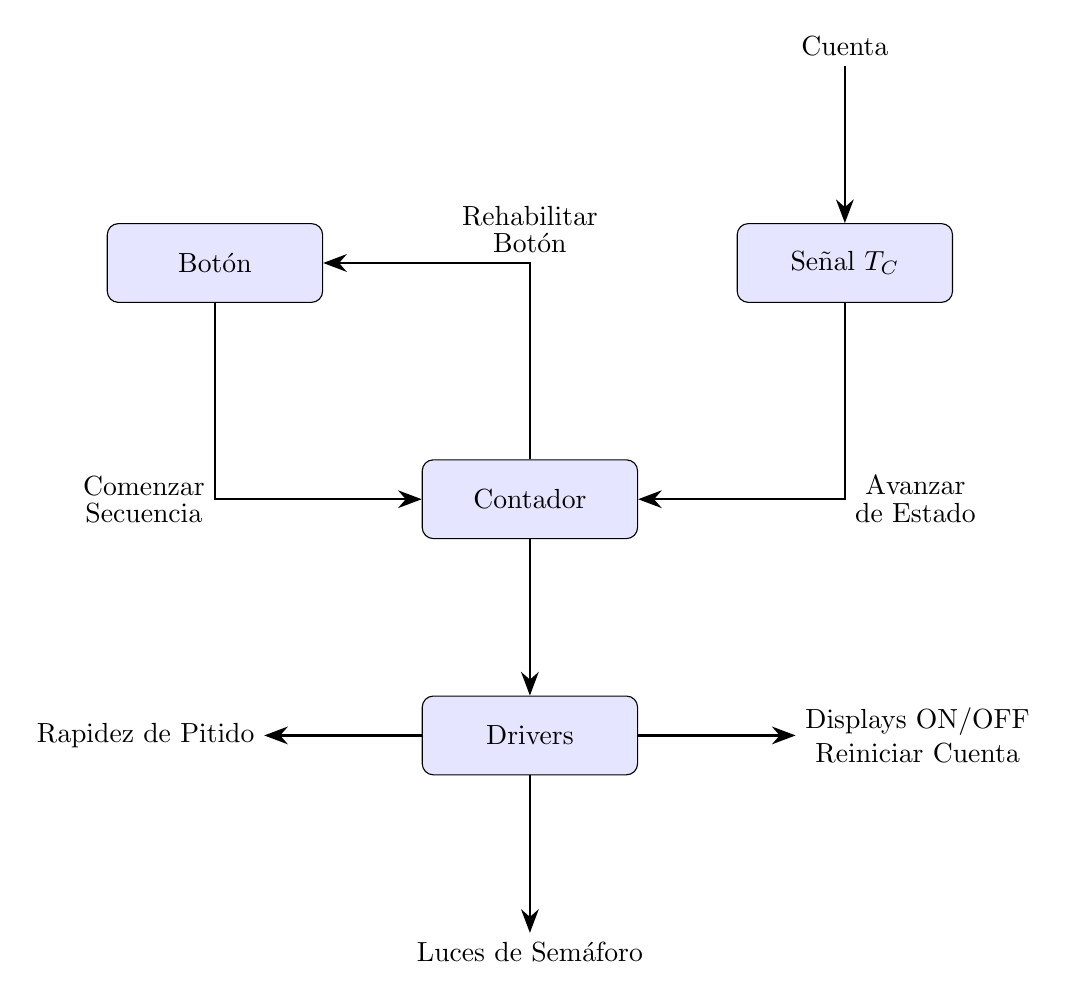
\begin{tikzpicture}[
    node distance=2cm,
    block/.style={rectangle, draw, fill=blue!10, text width=2.5cm, text centered, rounded corners, minimum height=1cm},
    arrow/.style={thick, -{Stealth[length=3mm]}}
]

\node (boton) [block] at (0,0) {Botón};
\node (contador) [block] at (4,-3) {Contador};
\node (tc) [block] at (8, 0) {Señal $T_C$};
\node (drivers) [block] at (4, -6) {Drivers};

\node (cuenta) [above =of tc] {Cuenta};

\node (luces) [below =of drivers] {Luces de Semáforo};
\node (displays) [right =of drivers] {\shortstack{Displays ON/OFF \\ Reiniciar Cuenta}};
\node (audio) [left =of drivers] {Rapidez de Pitido};


\draw [arrow] (boton.south) |- node[left] {\shortstack{Comenzar \\ Secuencia}} (contador.west);
\draw [arrow] ([xshift=0pt]contador.north) |- node[above] {\shortstack{Rehabilitar \\ Botón}} (boton.east);
\draw [arrow] (tc.south) |- node[right] {\shortstack{Avanzar \\ de Estado}} (contador.east);

\draw [arrow] (cuenta.south) -- (tc.north);

\draw [arrow] (contador.south) -- (drivers.north);

\draw [arrow] (drivers.west) -- (audio.east);
\draw [arrow] (drivers.south) -- (luces.north);
\draw [arrow] (drivers.east) -- (displays.west);

\end{tikzpicture}

\end{document}
